\chapter{Design}~\label{cha:design}
Before initiating detailed design work, it was decided this project would be a web application accessible via a browser. This approach offers several advantages, such as cross-platform compatibility, ease of access (requiring only a browser), scalability, and the ability to leverage existing web technologies~\cite{6822300}. With this established, a plan was formulated, encompassing architectural decisions, technology stack selection, and the definition of testing criteria.

\section{Architecture}
The system architecture defines the overall structure of the project and the communication between its components. For this project, two architectural approaches were considered: a monolithic architecture and a microservices-based architecture.

\subsection{Monolithic}
For this project, the monolithic approach offers several benefits. With all code centralised within a single framework, development is simplified, and debugging becomes more straightforward. Additionally, initial deployment is less complex since only one program needs to be managed once development is complete~\cite{9109514}.

However, the monolithic design has its drawbacks. As the system grows, maintaining a large, integrated codebase can become increasingly challenging; test suites may grow more complex and time-consuming to execute. During deployment, a single fault could potentially bring down the entire system, resulting in a complete loss of service. Similarly, even minor updates would require redeploying the entire monolith, increasing the risk of downtime. Moreover, this approach does not scale as effectively for web applications; as user demand increases, the need to redeploy the monolith frequently to manage higher request volumes becomes a significant concern~\cite{9109514}.

Although the scope of this project is small and so the drawbacks of a monolithic approach would have minimal impact, it was determined that the project should be designed to be fully scalable. With the potential for future growth in features and user base, the limitations inherent in a monolithic architecture would eventually become a hindrance in this scenario. Consequently, the monolithic approach was ruled out in favour of a more scalable architectural model.

\begin{figure} [H]
    \centering
    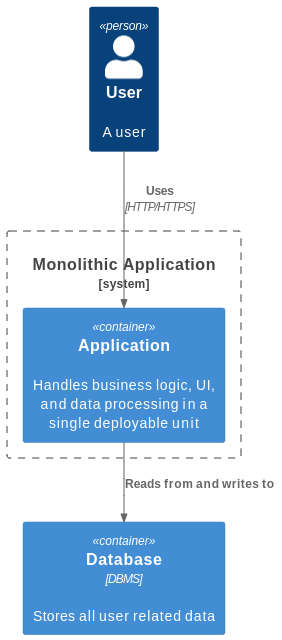
\includegraphics[width=0.35\linewidth]{figures/monolithic_arch.png}
    \caption{A potential architecture for a monolithic approach}
~\label{fig:monolith-arch}
\end{figure}

\subsection{Microservices}
The alternative approach examined was the use of microservices. In this architecture, the application's functionality is divided into separate services that communicate with each other using standardised protocols such as HTTP.\@

The primary benefits of this approach pertain to deployment and maintenance. Once deployed, the system can be scaled more efficiently—only those services experiencing high demand need to be replicated, which is significantly faster and more resource-efficient than scaling a monolithic system. Additionally, maintenance is simplified because each service operates independently; developers can focus on individual components without needing a comprehensive understanding of the entire system something that can become difficult even in small systems like this project.

However, the increased complexity of managing multiple services means that initial deployment is more challenging. Configuring the different addresses for inter-service communication can prove to be difficult, and each service requires setup that would only need to be completed once for a monolith. Nonetheless, once this initial configuration is completed, development within a microservices architecture becomes as straightforward as working with a monolithic architecture.

\begin{figure} [H]
    \centering
    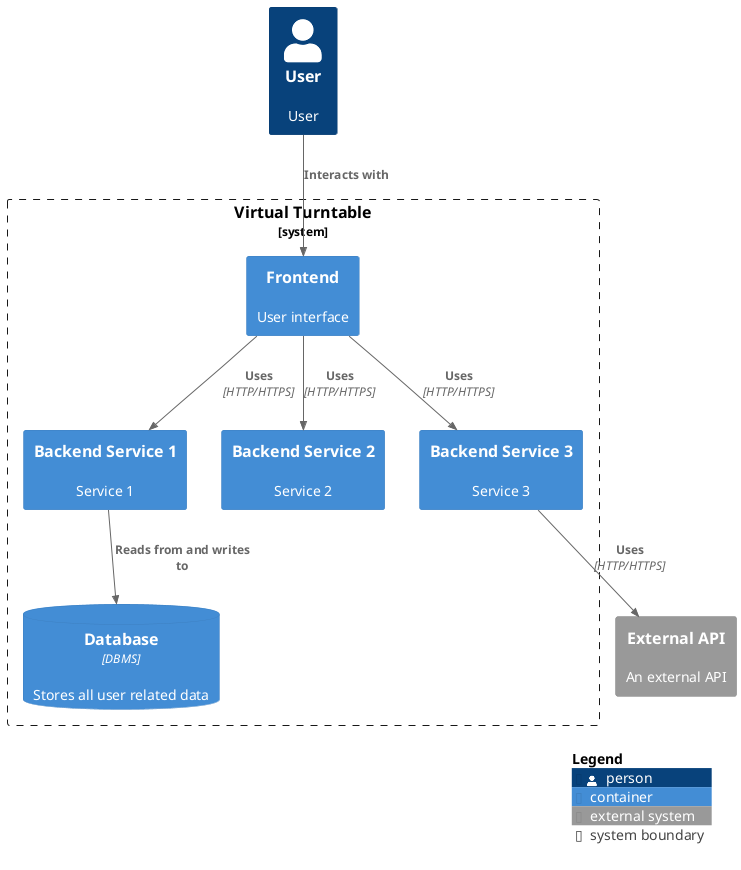
\includegraphics[width=0.5\linewidth]{figures/microservices_arch.png}
    \caption{A potential microservices design with three backend services}
    \label{fig:microservices-arch}
\end{figure}

\subsection{Final design}
The final design employs a microservices approach alongside a backend-for-frontend (BFF) design pattern. In this pattern, a dedicated backend service is created for each type of frontend application, such as desktop or mobile, ensuring that each backend caters specifically to a specific interface’s requirements. This pattern leverages the benefits of a microservices architecture and helps to maintain complexity by isolating functionality~\cite{BFF}. Details about each microservice are described in Section~\ref{sec:backend-design}.

\begin{figure} [H]
    \centering
    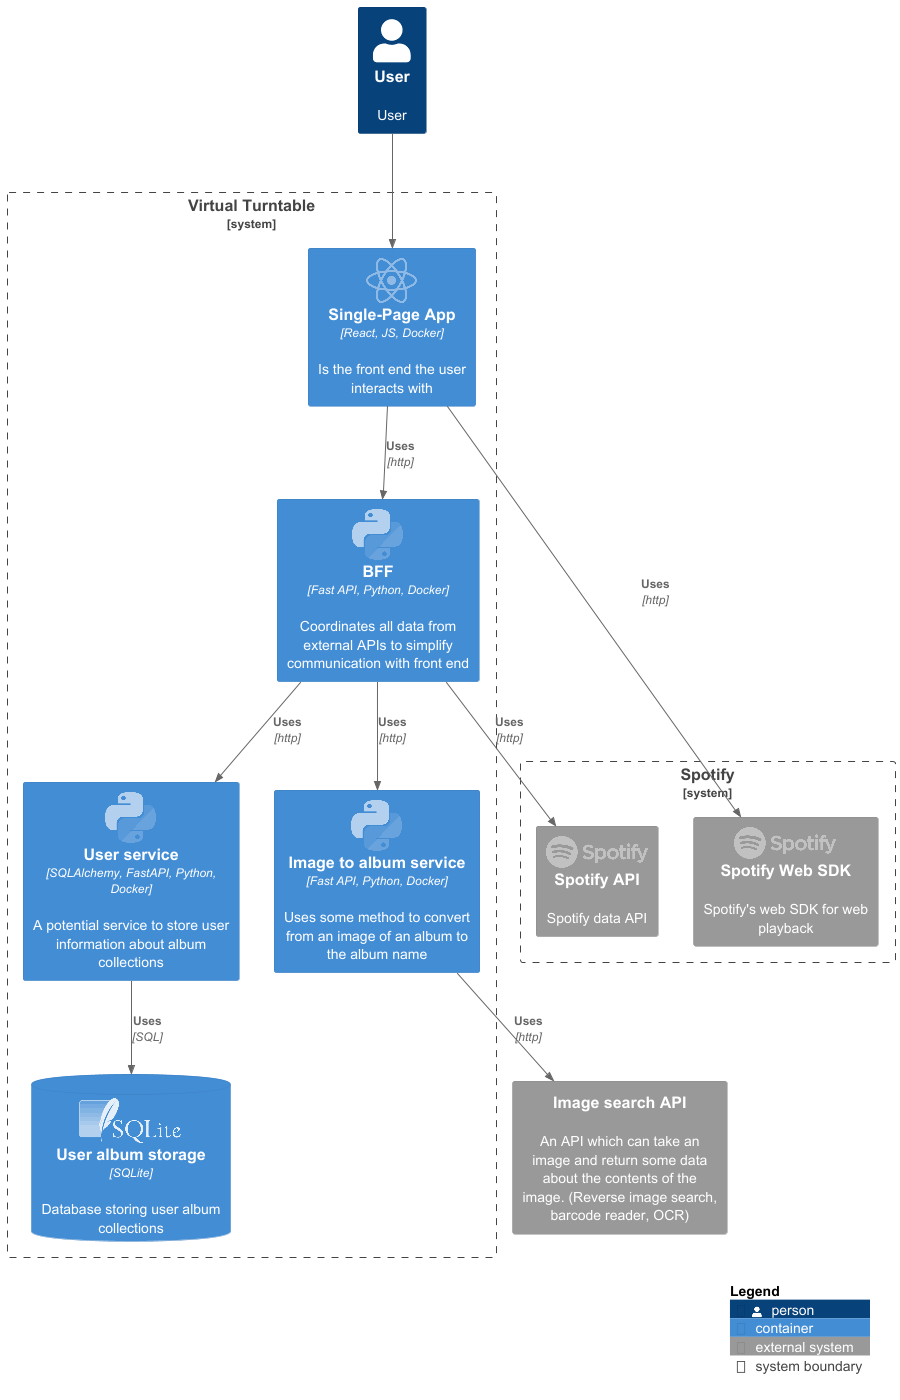
\includegraphics[width=0.5\linewidth]{figures/final_arch.png}
    \caption{The final architecture including technologies and external APIs}
    \label{fig:final-arch}
\end{figure}


\section{Technologies}
\subsection{FastAPI}
FastAPI is a Python web framework for building APIs, offering automatic input validation via Pydantic and seamless relational database integration with SQLAlchemy~\cite{FastAPI}. Compared to other popular frameworks like Django and Flask, FastAPI was particularly well-suited for this project due to its lightweight nature and built-in compatibility with these technologies. This combination provided an optimal balance between ease of setup and feature-rich functionality.

FastAPI was extensively utilised to develop all backend services in this project. Its straightforward setup allowed for rapid initial development, enabling quick implementation of basic functionality.

The backend primarily operated through individual API endpoints, which the frontend called to retrieve data as needed. Additionally, WebSockets facilitated asynchronous server-to-client communication, ensuring users were promptly notified of backend events, such as collections being shared with them.

\subsection{React}
React is a JavaScript library for building interactive web interfaces~\cite{React}. Its modular, component-based architecture was particularly beneficial in this project, enabling component reuse across multiple pages and reducing code duplication. A key advantage of this approach is the availability of extensive component libraries that provide pre-built functionality and styling for low-level elements, such as buttons. This allowed development efforts to focus on the application's bespoke features.

For this project, the HeroUI component library was utilised, offering a set of pre-designed components that were assembled into larger, more complex UI elements to create the final application.

React also managed the application's state and handled backend requests as needed. This enabled backend services to remain stateless, reducing complexity and improving scalability.

\subsection{Docker}
Docker is a platform for containerising applications, allowing them to run in isolated environments while communicating through specified exposed ports~\cite{DockerDocs}. This approach is a standard practice in modern web development and is widely supported by cloud providers, simplifying deployment and providing a consistent environment across different platforms.

For this project, Docker enabled fast and efficient deployment. Cloud providers could autonomously build and run the application when supplied with the codebase and Dockerfile. Additionally, for development, the containerised system could be easily executed on any device running Docker, eliminating the need for manual environment configuration.

All backend services and frontend, were containerised using Dockerfiles and deployed to a cloud provider, ensuring a scalable and reproducible deployment process.

\subsection{Spotify API And Web Playback}
The music service Spotify offers a suite of APIs for music-related services, including search and playback functionalities that matched the core features of this project~\cite{SpotifyAPI}. Given the impracticality of maintaining an independent album database, offloading the responsibility of maintaining a library of albums and music to Spotify was a logical choice.

Specifically, the search API was used to identify albums, while the playback API enabled streaming of the selected content.

However, a key limitation of this approach is that the playback API requires a Spotify Premium subscription. Though, as the Spotify API mandates user authentication via a Spotify account, this requirement allows the Spotify account to serve as the user account for the application, thereby reducing security concerns related to the storage and management of user data.

\subsection{Reverse Image Search}~\label{sec:reverse-image-search}
Reverse image search is a form of content-based image retrieval that uses an image as the query to retrieve related results. This process involves extracting feature vectors, using algorithms such as SIFT, and comparing these against a collection of previously indexed images to return the closest matches~\cite{Gaillard2017LargeSR}.

In this project, reverse image search functionality was implemented to identify albums from images uploaded by users. Recognizing that maintaining an up-to-date, in-house database of album covers would be impractical, it was decided early on to leverage an external API.\@ Two reverse image search APIs were evaluated: Google and Bing. Although Bing's API was simpler to integrate, it frequently failed to accurately identify albums—even from images that were already indexed by Bing's image search. In contrast, Google's API demonstrated a much higher reliability in album identification. Given the critical importance of accurate album retrieval for the project, the Google API was ultimately chosen.

Compared to other methods for recognizing albums from images, such as optical character recognition (OCR) or barcode scanning, reverse image search was selected for its robustness. OCR can be unreliable when album covers feature stylised text or lack text entirely and barcode scanning, though dependable, requires a barcode to be present. This requirement is problematic, particularly since vinyl records may predate the widespread use of barcodes.

\subsection{Google Cloud}
Google Cloud is a suite of cloud services offered on a pay-as-you-use basis~\cite{GCP}. In this project, two specific services were utilised: the reverse image search API and Google Cloud Run. The reverse image search API was employed to identify albums from images uploaded by users, as detailed in Section~\ref{sec:reverse-image-search}. Google Cloud Run was used to build and host the application, running in Docker containers.

Although multiple cloud providers were available, Google Cloud was selected following the adoption of Google's reverse image search API.\@ For convenience, hosting the application on Google Cloud was simpler as it eliminated the need to manage services across different providers.

\section{Frontend}
The frontend is the user facing part of the application, because of this it needed to be designed with the knowledge that users have a wide range of abilities and needs. This meant that the user interface needed to be intuitive and easy to use.

A `multipage' design approach was selected for the application as this separates the application into sections, so the user is not overloaded on a single page. This could have been implemented in two ways, a router design where the separate pages are loaded as the user navigates the application or a single page app where the screens are different `tabs'. The former would have been simpler as there would be little to no implementation to link the pages together, but it was decided to implement later. This was done as it was thought this would provide a more fluid user experience where the user could easily switch between different views. This also had the benefit of allowing music playback to continue even as the user navigates the application.

\subsection{Principles}
An easy way to ensure that the user interface is well-designed is to follow a set of principles. A good example of these would be Shneiderman's eight golden rules of interface design~\cite{Shneiderman} which were used as a guideline in this project to ensure that the user interface was intuitive and easy to use. %These rules are as follows:
\iffalse
\begin{itemize}
    \item Strive for consistency
    \begin{description}
        \item[] The design should be consistent throughout the application, components should look and behave the same way wherever they are used.
    \end{description}
    \item Seek universal usability
    \begin{description}
        \item[] Users have diverse needs and abilities, so the design should not exclude any potential users.
    \end{description}
    \item Offer informative feedback
    \begin{description}
        \item[] There should be feedback to user actions, such as dialogue boxes, loading spinners, or page transitions.
    \end{description}
    \item Design dialogues to yield closure
    \begin{description}
        \item[] Actions in the application should have some sort of logical structure
    \end{description}
    \item Prevent errors
    \begin{description}
        \item[] Users should not be allowed to do things that would cause errors, for example buttons should be disabled if they should not be used.
    \end{description}
    \item Permit easy reversal of actions
    \begin{description}
        \item[] Users should be able to undo actions, for example, a confirmation dialogue before deleting something.
    \end{description}
    \item Keep users in control
    \begin{description}
        \item[] Users should feel the application is acting as they intend it to, there should be few surprises, and behaviour should be predictable.
    \end{description}
    \item Reduce short-term memory load
    \begin{description}
        \item[] There should only be a small amount of information of the screen at one time, and the user should not have to remember things from one screen to another.
    \end{description}
\end{itemize}
\fi

\subsection{Wireframe mockups}
Prototyping the user interface provides a rapid way to visualize the application, enabling design evaluations without the need to write any code~\cite{WILSON1988859}. This approach proves especially beneficial during the early stages of development, when the design remains flexible and can be easily modified. In this project, wireframe mockups were selected for their low-fidelity nature, which allowed fast iteration on design.

Across all mockups, a consistent navigation bar is present at the top of the screen, allowing for straightforward navigation among the application's various pages.

\subsubsection{Play Screen}
Figure~\ref{fig:play_screen_mockup} depicts the mockup of the play screen, where users control music playback. Essential functionality implemented here includes buttons to play, pause, skip forward or backward, adjust the track position, and manage volume. Fitting with a modern streaming service, individual tracks can be played from the album, even though this would not be commonly done with a physical turn table.

The screen is also designed to incorporate elements of a physical turntable as part of the theme. Mainly the spinning vinyl seen in the centre.
\begin{figure} [H]
    \centering
    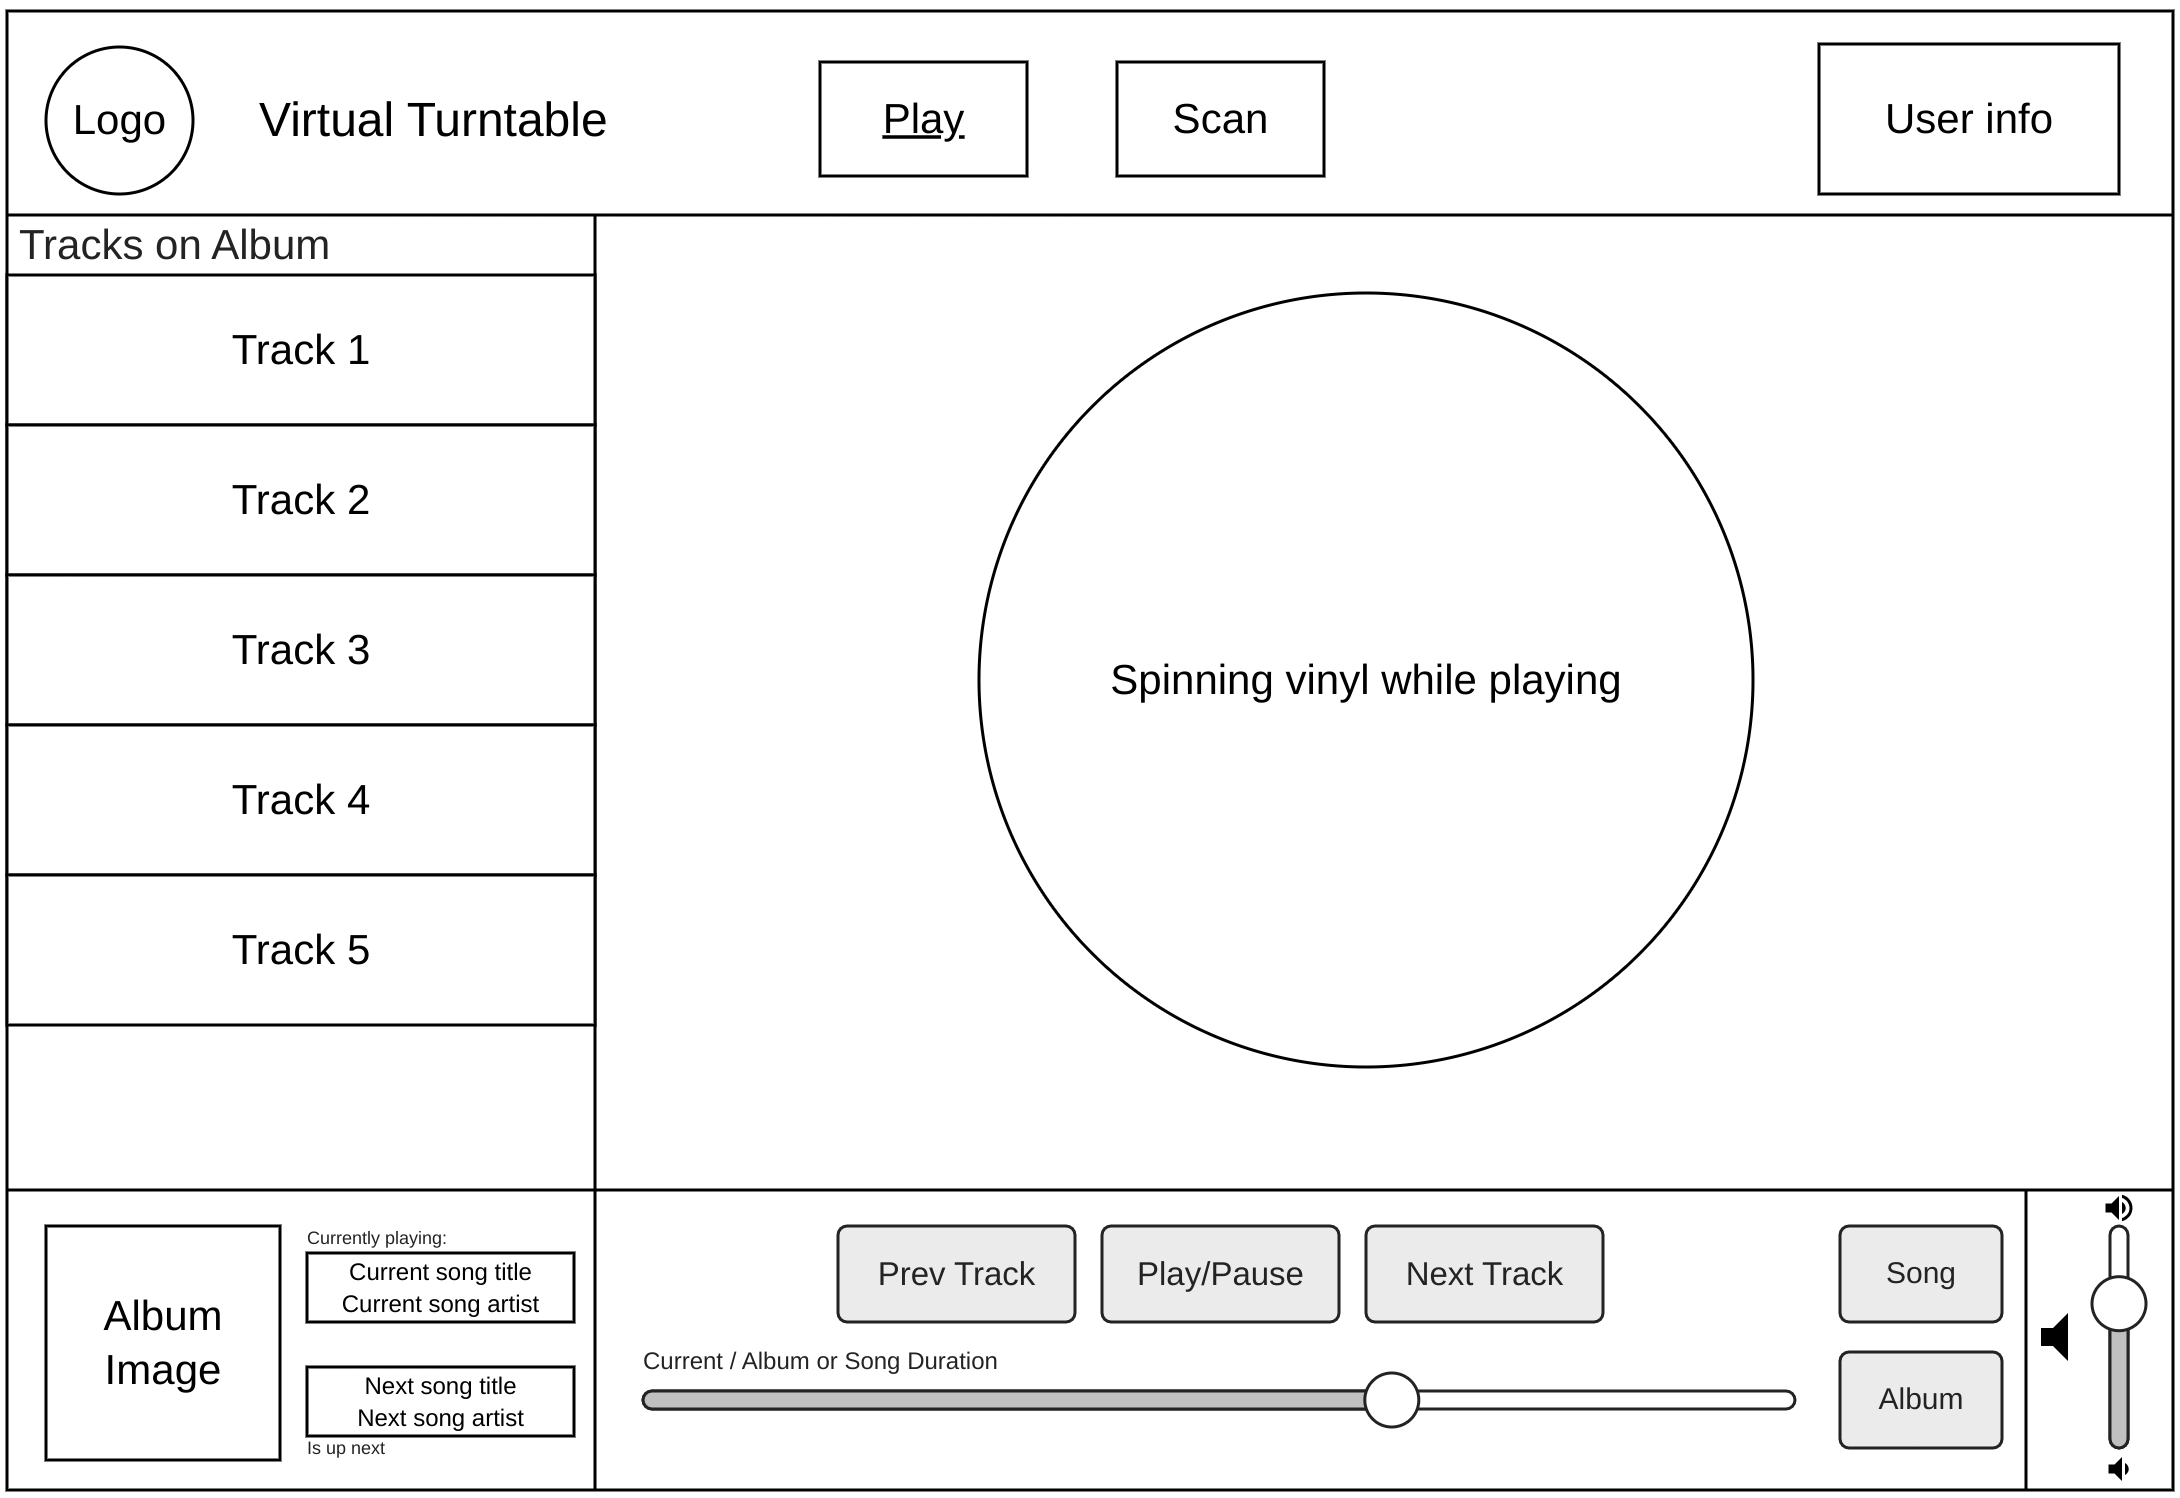
\includegraphics[width=0.6\linewidth]{figures/play_screen_mockup.png}
    \caption{The play screen wireframe mockup}
    \label{fig:play_screen_mockup}
\end{figure}

\subsubsection{Scanning Screen}
Figure~\ref{fig:scan_screen_mockup} shows the scanning screen, where users can upload images of album covers to identify the corresponding album. It also displays the logged-in user’s existing album collection, allowing quick selection of albums already scanned. The confirmation dialogue (shown on the left) enables users to confirm the identified album or reject it if incorrect.

\begin{figure} [H]
    \centering
    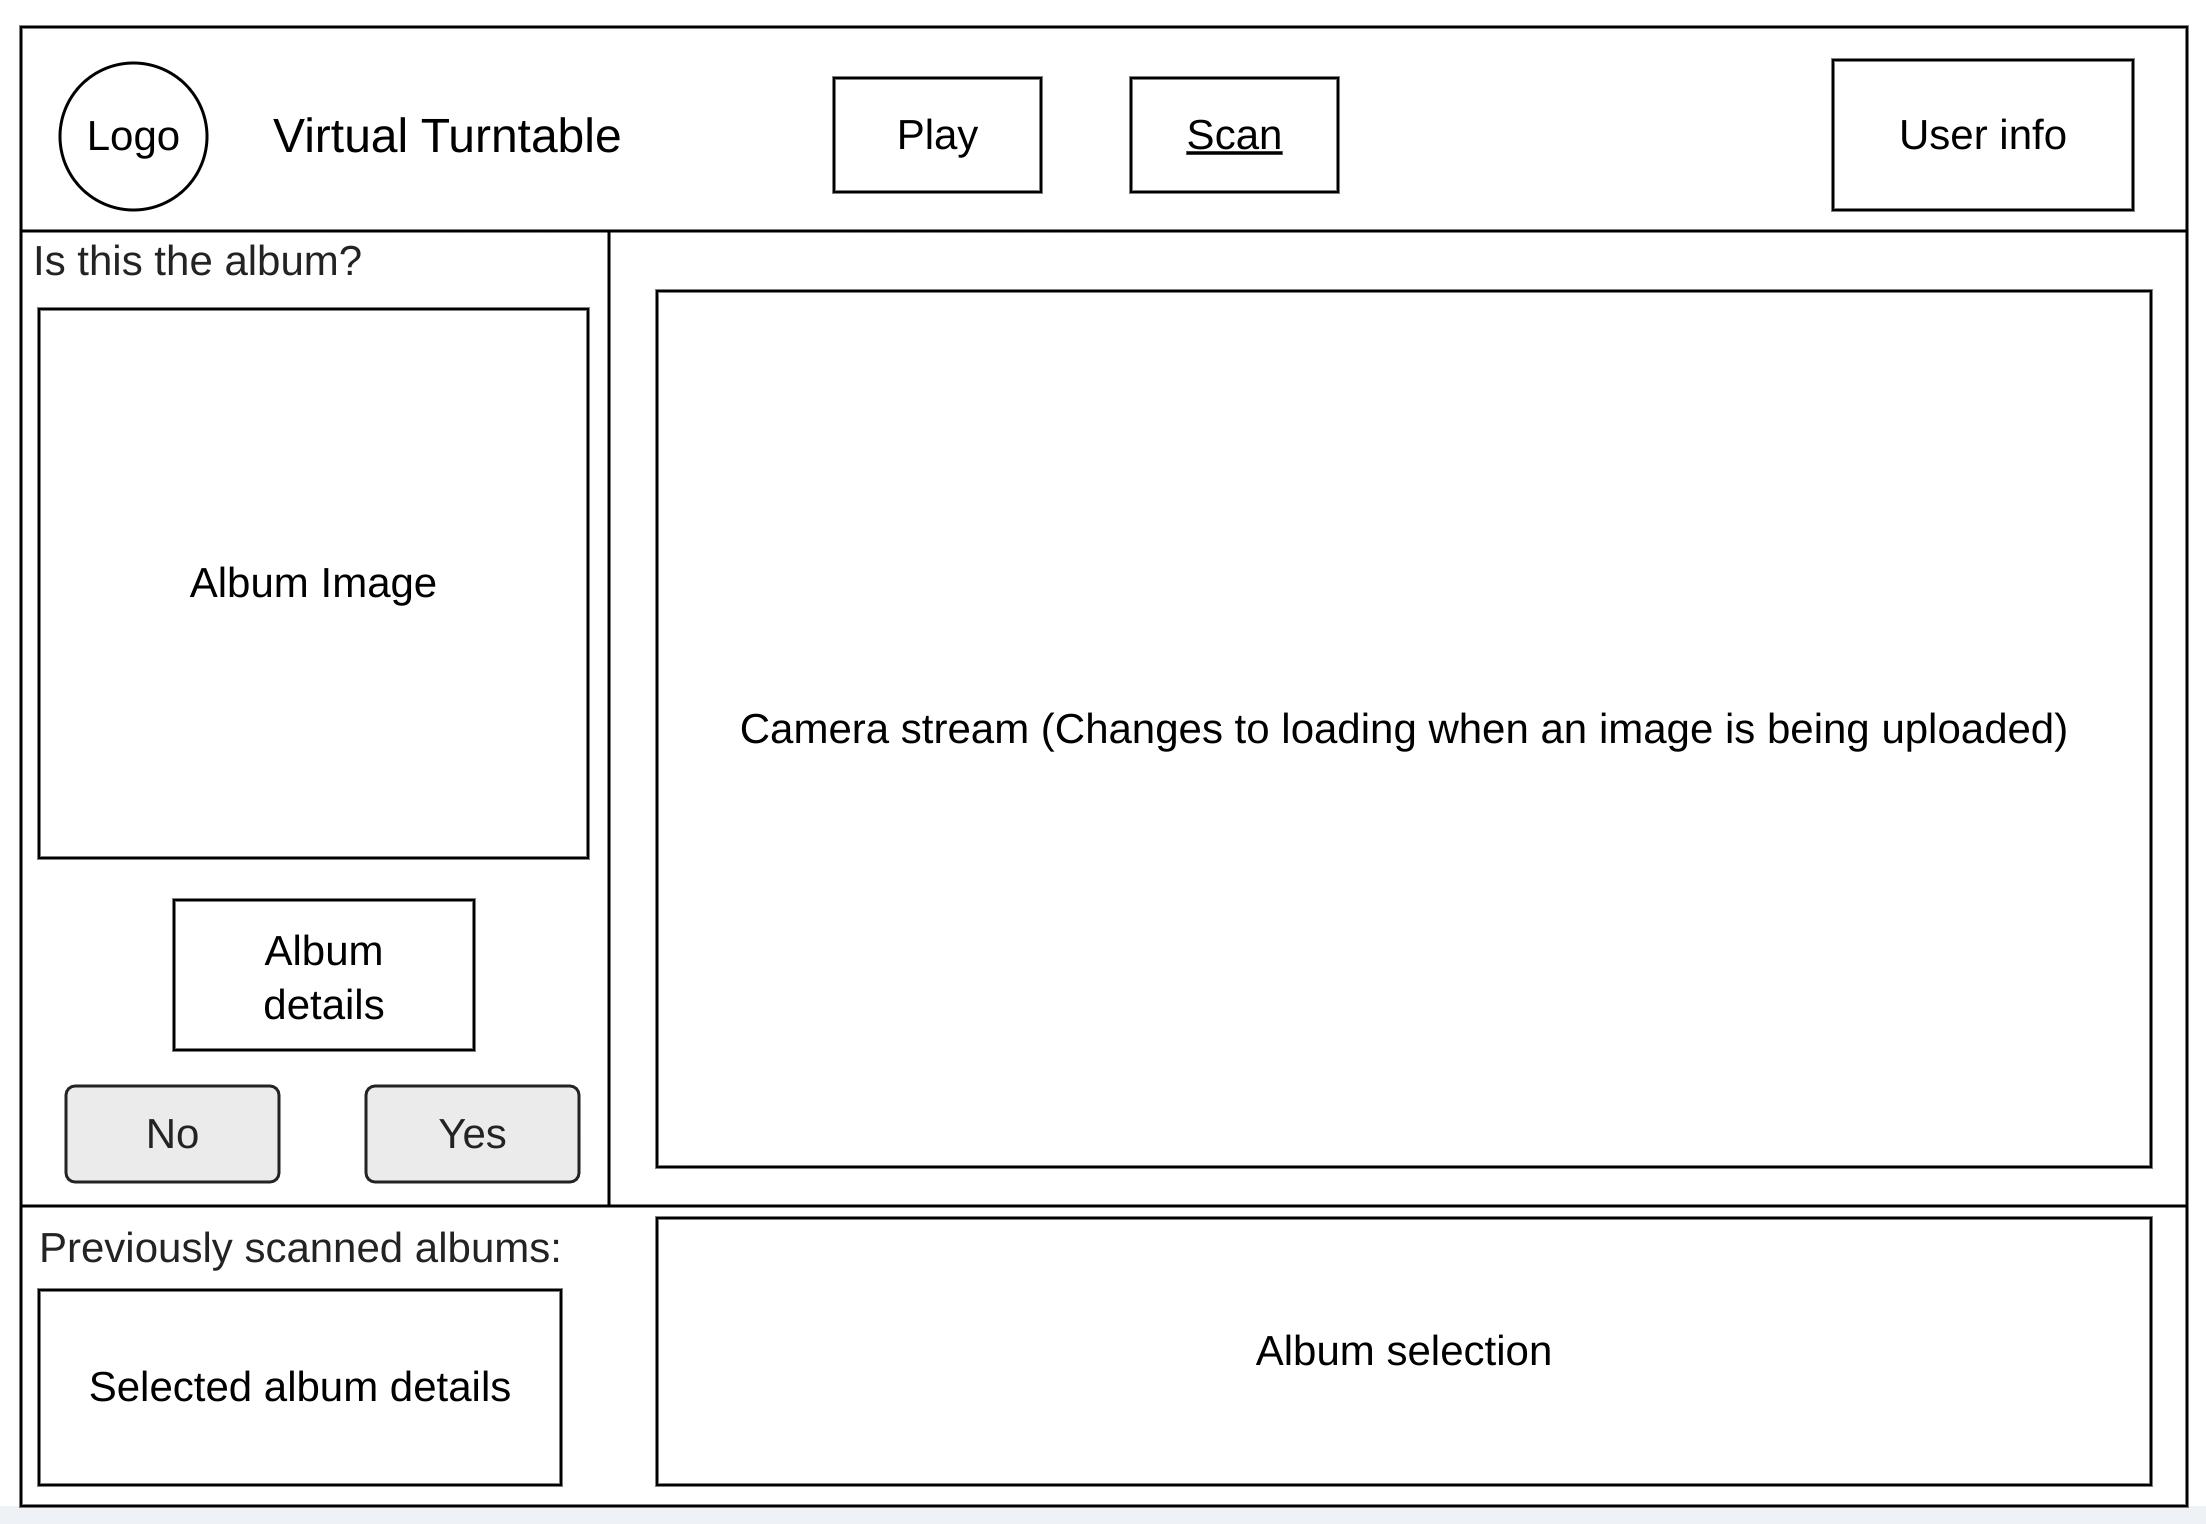
\includegraphics[width=0.6\linewidth]{figures/scan_screen_mockup.png}
    \caption{The scanning screen wireframe mockup}
    \label{fig:scan_screen_mockup}
\end{figure}


\subsubsection{Social Screen}
Figure~\ref{fig:social_screen_mockup} shows the social screen, where users can view collections belonging to others shared directly with them or made public by other users. This feature aimed to add a sense of social interaction among users and allow for the discovery of new music.

%Initially, albums were displayed in columns, but this layout proved limiting for users with extensive collections as it required excessive scrolling. Moreover, this featured presented an opportunity to capture the feel of browsing through a physical record store, prompting a revision of the layout to accommodate larger collections more intuitively. TODO: ref later section about development

\begin{figure} [H]
    \centering
    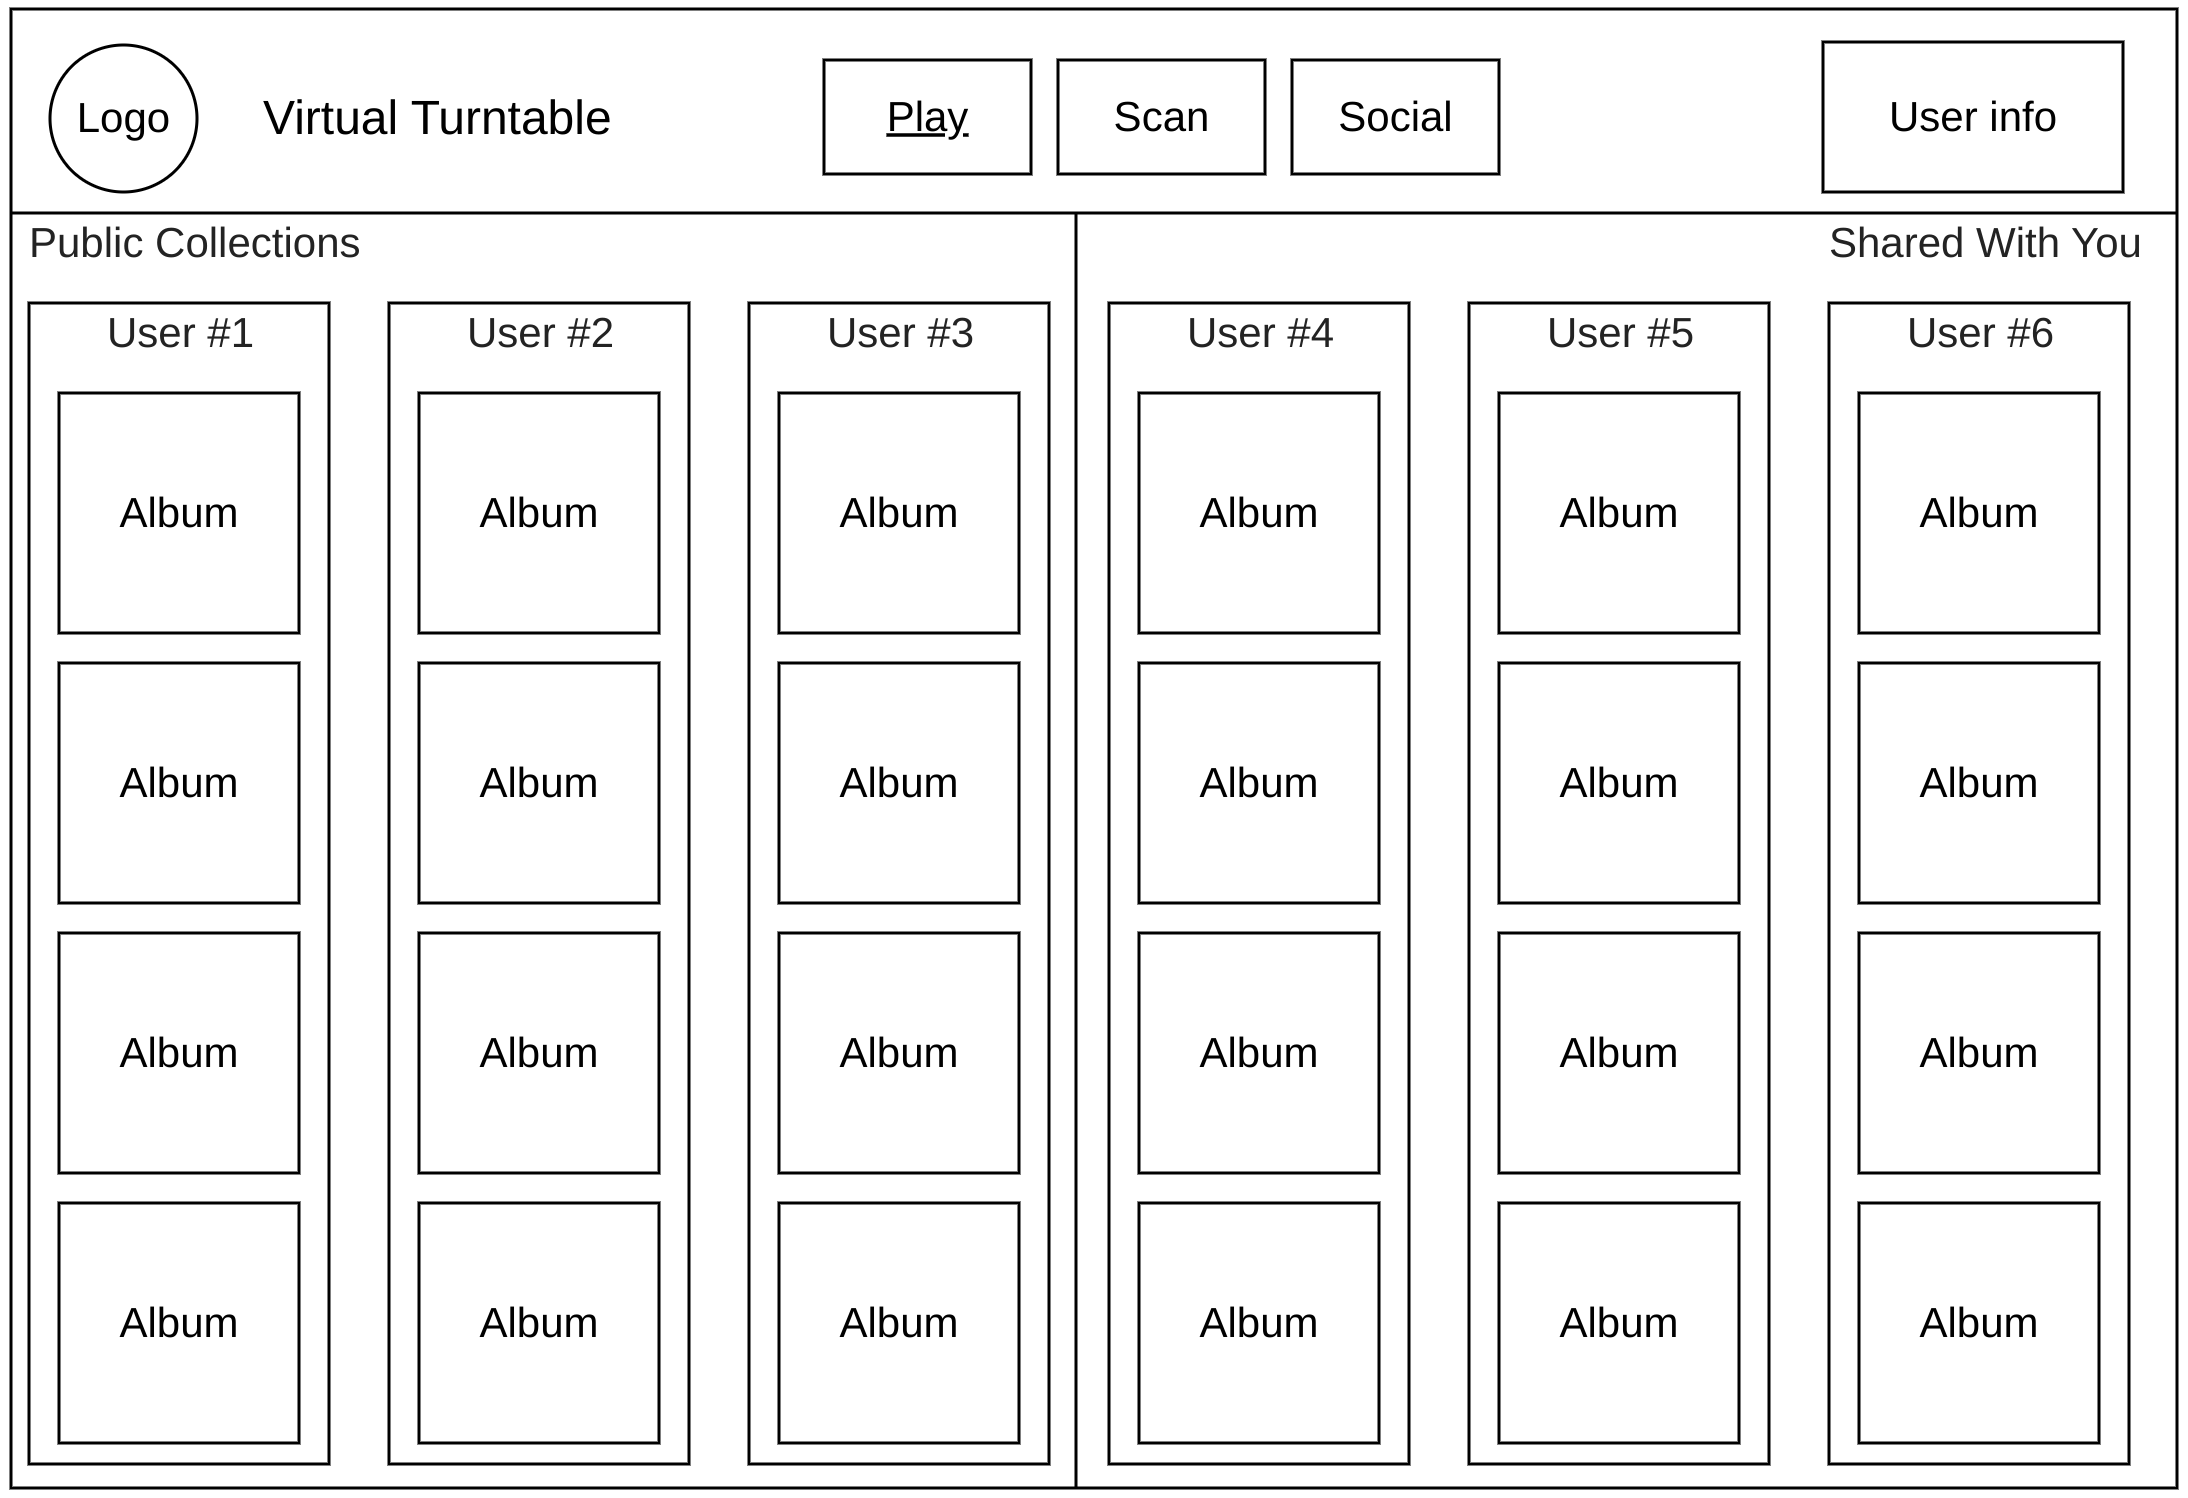
\includegraphics[width=0.6\linewidth]{figures/social_screen_mockup.png}
    \caption{The social screen wireframe mockup}
    \label{fig:social_screen_mockup}
\end{figure}

\section{Backend}~\label{sec:backend-design}
The backend for the project would responsible for handling all business logic and data handling. It would mostly respond to API calls from the frontend except in cases where the backend would need to asynchronously push data to the frontend. This would be done using WebSockets.

\subsection{Microservices split}
As a microservices approach was adopted, the backend operations were divided into multiple services. As described in Section~\ref{fig:final-arch}, it was decided to use a BFF (Backend for Frontend) pattern for one of these services. The remaining functionality was split into two services; one service handles the conversion of user-uploaded images into album data, while another manages all user-related data storage.

\subsubsection{BFF}
The BFF acts as a middleman between the frontend and various backend services, often mirroring the endpoints of those services. Its main responsibility is to manage the data returned to the frontend. As this project is focused solely on a desktop web application, so the patterns potential to tailor data for different platforms was not fully utilised. However, if the application were later expanded to include additional platforms, the BFF could selectively limit data returned to given devices if it did not require it.

The BFF also handles the WebSocket connections to the frontend, allowing the backend to push data to the frontend when necessary. This is particularly useful for notifying users of new shared collections or other events that require immediate attention.

\subsubsection{Image to Album}
This service was the smallest of the three, encapsulating a very specific functionality. It included endpoints responsible for identifying albums from various inputs, such as images of the album, allowing different methods, such as OCR or reverse image search to be handled through separate endpoints with the caller choosing which to use. Along with that the service also hosted a way to search for albums using Spotify's API as a method to return an exact album from a guess that might have been generated by an identification method.

Separating these functions from the rest of the application’s services means users could still listen to their existing collections in the event that this service going down.

\subsubsection{User Data}
This service was to handle all tasks related to user data such as collections and sharing. It would do this by interacting with a database detailed in Section~\ref{sec:database}. Each endpoint would be responsible for editing the data in the database in some way such as creating a user or sharing a collection.

\subsection{Database}~\label{sec:database}
This application could have been implemented as a stateless application which would  mean there was no capability to persist data across sessions. However, such an approach would limit functionality as there could be no form of personalisation for individual users. Since a Spotify account was already required for music playback, linking user data to that account became a logical next step, enabling data persistence across sessions.

\subsubsection{SQL vs NoSQL}
SQL databases are widely used in enterprise environments due to their reliability and consistency. However, relational databases are not necessarily optimal for web applications that require high scalability and availability~\cite{GANESHCHANDRA201513}. In contrast, NoSQL databases are designed with scalability and availability in mind~\cite{NoSQL}, often making them more suitable for such applications.
Although a NoSQL database like MongoDB would have been a good choice for this project, a SQL database was selected for its easy integration with FastAPI and SQLAlchemy. This meant quicker development and cleaner code, despite not being the most inherently scalable option.

\subsubsection{Diagram}
\begin{figure} [H]
    \centering
    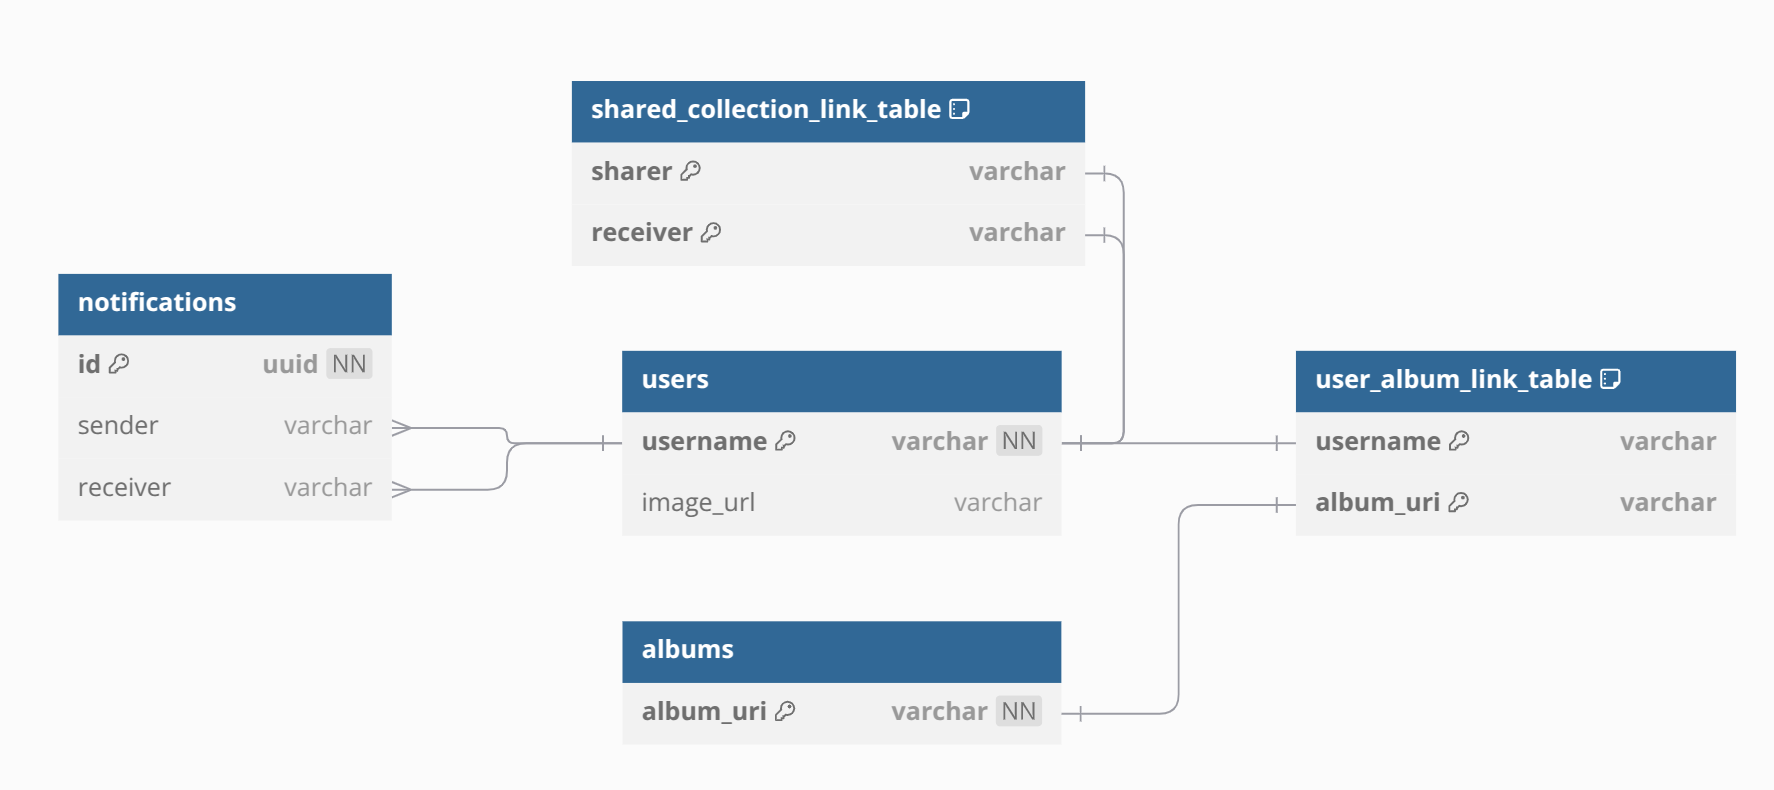
\includegraphics[width=0.6\linewidth]{figures/db_diagram.png}
    \caption{A diagram of the database using crow's foot notation}
    \label{fig:database-diagram}
\end{figure}

Figure~\ref{fig:database-diagram} shows the database design. User are stored with their Spotify usernames as primary keys as Spotify guarantees unique usernames. This allows data in other tables to be linked through each user’s username. Collections are represented with a link table that captures the many-to-many relationship between users and albums. A similar link table structure is used to manage the sharing of collections, tracking which users have shared access with each user. In addition, notifications regarding newly shared collections are stored in a separate table. These have to be stored between sessions as not all users are logged in simultaneously so, upon login, the user's notifications are fetched and displayed.

\subsubsection{DBMS Choice}
Since the choice was made to use a relational database, a specific relational database management system had to be selected even though the use of SQLAlchemy abstracts many of the differences among various DBMSs allowing one system to be swapped out for another with no code changes. The only notable exception is that SQLite does not enforce foreign key constraints by default, requiring manual enablement.

Originally, SQLite was chosen because, as since it's a file-based database, it could be easily stored within the Docker container running the user data service, which would simplify deployment by reducing the number of containers. However, as the project grew, the need for concurrent database access became apparent which SQLite does not support. Because of this the decision was made to switch to either MySQL or PostgreSQL, both of which support concurrent access. For the purposes of this project, the differences between these two systems were minor. PostgreSQL was selected since it is open-source, which reduces the risk of support being dropped in the future.

\subsection{Security}
Security is an important consideration for any web application, since functionality and access to user data is exposed to the internet. Although the stored user data in this project is not particularly sensitive, it should still be safeguarded. To ensure this measures had to be implemented for each backend service.

\paragraph{BFF} The BFF represents the largest potential security risk, as it is the only service that directly interacted with the frontend and therefore exposed to the public internet. To mitigate this risk, the BFF used authentication to verify requests to all endpoints related to user data. The exact details of the implementation of this are specified in Section~\ref{sec:backend-security}.

\paragraph{Image-to-Album \& User Data Services} These services operate behind the BFF and only need to accept requests from that single, predictable source. Because of this, these services are designed to reject any requests originating from any external sources ensuring that only valid requests are processed.

\section{Testing}~\label{sec:test-design}
Defining the tests and success criteria prior to development was important to ensure that the project was built to meet these objectives, rather than retrofitting tests to match the final product. For most of the criteria listed in Section~\ref{sec:objectives}, it was necessary to establish tangible measurements to determine whether those criteria had been met.

\subsection{Primary Features}
For the two discussed primary features these tests were defined:
\begin{itemize}
    \item The application should correctly identify albums with at least $95\%$ accuracy. This functionality must be accurate but the threshold of $95\%$ is an arbitrary value chosen as it is expected the system will reach a high but not perfect level of accuracy.
    \begin{description}
        \item[Verification:] Take a set of input images, modified to be of both poor and good quality, and calculate the accuracy of the system. It is important that, as the application will likely rely on external APIs, this functionality the accuracies of any APIs are taken into account.
    \end{description}
    \item The application should play an album from start to finish without interruption.
    \begin{description}
        \item[Verification:] Play a set of albums on the application and verify that all play without interruption.
    \end{description}
\end{itemize}

\subsection{User Interface}~\label{sec:ui-tests}
For criteria relating to the user interface it is harder to be objective as the quality of the interface is subjective. To determine if the objectives were met, a sample of users would need to be asked to use the application and provide feedback on the interface. This feedback could then be used to determine if the interface was easy to use and visually appealing as well as understanding if users liked and found the saving and sharing features useful.

For this purpose the following survey was put together consisting of seven questions:
\begin{itemize}
    \item How easy was the application to use? (1 - 10)
    \item How visually appealing was the application? (1 - 10)
    \item Did you understand that listening to an album saved it to a collection associated with your account? (Yes/No)
    \begin{itemize}
        \item If yes, how useful did you find the collection saving feature? (1 - 10)
    \end{itemize}
    \item Did you understand that you could share your album collection with other users and other users could share theirs with you? (Yes/No)
    \begin{itemize}
        \item If yes, how useful did you find the social features? (1 - 10)
    \end{itemize}
    \item Any extra comments? (Free text)
\end{itemize}

These questions cover the main objectives of the user interface and as such should provide a good indication of whether the objectives were met.

\subsection{Code Quality}
The last set of criteria, relating to good software development practices, are generally more objective and as such are more easily verifiable. For this the following tests were defined:
\begin{itemize}
    \item The codebase should maintain at least $95\%$ test coverage. This threshold is high enough it can guarantee much of the code is tested but not so high that it becomes difficult to maintain.
    \begin{description}
        \item[Verification:] Run all test suites and verify the line coverage and branch coverage exceed $95\%.$
    \end{description}
    \item All tests must pass successfully.
    \begin{description}
        \item[Verification:] Run all test suites and verify that all tests pass.
    \end{description}
    \item Code should be evaluated by linters and formatters to maintain consistency and quality.
    \begin{description}
        \item[Verification:] For Python code, run ruff for formatting and Pylint for linting. For typescript run Biome for both formatting and linting. Both should pass without errors.
    \end{description}
    \item A continuous deployment system should automatically redeploy the application following any code change.
    \begin{description}
        \item[Verification:] Push a change to the repository and verify that the application is redeployed with the change in place.
    \end{description}
    \item An automated system should be in place to update dependencies.
    \begin{description}
        \item[Verification:] An automated tool for dependency management should be configured on the repository to run at a given interval.
    \end{description}
\end{itemize}

Most of these criteria can be met using tools such as GitHub Actions, which can run tests on each commit, and trigger application deployments. Dependabot can be used to scan the repository’s dependencies and update them as new releases become available. Additionally, linters and formatters can be executed as pre-commit hooks, preventing code below a defined quality threshold from being committed to the repository.

A side effect of having high test coverage is that there is a reduced risk associated with dependency updates, since tests help verify that no functionality has been broken by the update.
